\section{Galilean transformation}
    An \emph{inertial frame} is one in which the law of inertia holds good.
    \begin{itemize}
    	\item An ideal inertial frame is a coordinate frame of reference which is fixed in space with respect to the fixed stars.
    	\item A set of coordinate axes attached to the Earth may be regarded as an \emph{almost }inertial frame of reference.
    \end{itemize}
    An accelerating frame of reference is known as a \emph{non-inertial frame}.
    \begin{figure}[h!]
    	\centering
    	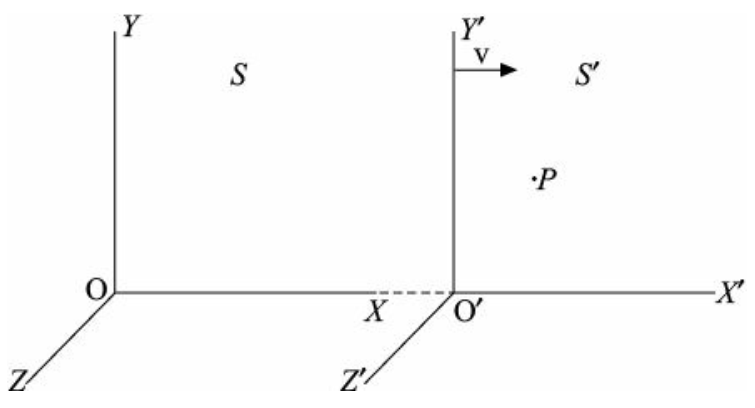
\includegraphics[width=0.55\textwidth]{figures/fig_galilean-transf-01.png}
    \end{figure}
    
    Consider two inertial frames $S$ and $S'$ with coordinate axes $xyz$ and $x'y'z'$ attached to them, with respective origins $O$ and $O'$ respectively. Let the frame $S'$ be moving with respect to $S$ with a uniform velocity $v$ along the $xx'$ axes as shown in the figure above. The origins of the two frames are assumed to coincide when $t=t'=0$.
    
    Let an event be taking place at $P$ whose coordinate with respect to $S$ be $(x,y,z,t)$, and with respect to $S'$ be $(x',y',z',t')$. Then these coordinates are related by the following \emph{Galilean transformation equations}:
    \begin{equation} \label{eqn:galilean-transf:posn}
    	\boxed{
    		\begin{aligned}
    			x'&=x-vt \\
    			y'&=y \\
    			z'&=z \\
    			t'&=t
    		\end{aligned}
    	}
    \end{equation}
    With the assumption that $\dv{t}=\dv{t'}$, we differentiate equation (\ref{eqn:galilean-transf:posn}) with respect to time to obtain the \emph{Galilean velocity transformations}:
    \begin{equation} \label{eqn:galilean-transf:vel}
    	\begin{aligned}
    		\dv{x'}{t'}&=\dv{t}(x-vt) \\
    		\dv{y'}{t'}&=\dv{y}{t} \\
    		\dv{z'}{t'}&=\dv{z}{t}
    	\end{aligned}
    	\implies\boxed{
    			\begin{aligned}
    				u_x'&=u_x-v \\
    				u_y'&=u_y \\
    				u_z'&=u_z
    			\end{aligned}
    	}
    \end{equation}
    Again we differentiate equation (\ref{eqn:galilean-transf:vel}) with respect to time to obtain the \emph{Galilean acceleration transformations}:
    \begin{equation} \label{eqn:galilean-transf:acc}
    	\begin{aligned}
    		\dfrac{\mathrm{d}^2x'}{\mathrm{d}t'^2}&=\dv[2]{x}{t} \\
    		\dfrac{\mathrm{d}^2y'}{\mathrm{d}t'^2}&=\dv[2]{y}{t} \\
    		\dfrac{\mathrm{d}^2z'}{\mathrm{d}t'^2}&=\dv[2]{z}{t}
    	\end{aligned}
    	\implies\boxed{
    		\begin{aligned}
    			a_x'&=a_x \\
    			a_y'&=a_y \\
    			a_z'&=a_z
    		\end{aligned}
    	}
    \end{equation}
    
    Because the directions of the unit vectors are parallel in both frames, we have $\vu{x}'=\vu{x}$, $\vu{y}'=\vu{y}$ and $\vu{z}'=\vu{z}$. Then from equation (\ref{eqn:galilean-transf:acc}), we find that
    \begin{align}
    	a_x'\vu{x}'+a_y'\vu{y}'+a_z'\vu{z}'&=a_x\vu{x}+a_y\vu{y}+a_z\vu{z} \nonumber\\
    	\implies \vb{a}'&=\vb{a} \label{eqn:galilean:acc-inv}
    \end{align}
    i.e. the acceleration of a particle remains invariant under a Galilean transformation.
    
    Multiplying equation (\ref{eqn:galilean:acc-inv}) by the mass $m$ of the particle, we have
    \begin{align}
    	m\vb{a}'&=m\vb{a} \nonumber\\
    	\implies\vb{F}'&=\vb{F} \label{eqn:galilean:F-inv}
    \end{align}
    Equation (\ref{eqn:galilean:F-inv}) implies that the force on a body remains invariant across inertial frames of reference.
    
    \textbf{Principle of Galilean-Newtonian relativity:} No inertial frame is special and all inertial frames are equivalent.
    	
    \subsection{The inadequacy of Galilean transformation}
    	As per Maxwell's electromagnetic theory, an electromagnetic (EM) wave propagates through free space with a constant speed of $c\approx\num{3e8}$ m/s.
    	
    	Then the wavefront of an EM wave emitted by a point source at $O$ would be spherical with a radius at time $t$ to be $ct$. Hence the spherical wavefront surface is given in the frame $S$ to be
    	\begin{align}
    		x^2+y^2+z^2&=\qty(ct)^2 \nonumber\\
    		\implies x^2+y^2+z^2-c^2t^2&=0 \label{eqn:spherical:S-01}
    	\end{align}
    	
    	For the Galilean-Newtonian principle to hold, we must have that the above equation is invariant between $S$ and $S'$, and so we must have
    	\begin{align}
    		x'^2+y'^2+z'^2-c^2t'^2&=0 \label{eqn:spherical:Sp}
    	\end{align}
    	
    	Substituting equations (\ref{eqn:galilean-transf:posn}) in equation (\ref{eqn:spherical:Sp}), we get
    	\begin{align}
    		\qty(x-vt)^2+y^2+z^2-c^2t^2&=0 \label{eqn:spherical:S-02}
    	\end{align}
    	
    	But equation (\ref{eqn:spherical:S-02}) is not identical to equation (\ref{eqn:spherical:S-01}). This inconsistency seems to suggest that there must be some special reference frame with respect to which the speed of light is $\num{3e8}$ m/s.
    	
    	In order to support this suggestion, it was assumed that light and other EM waves are mechanical waves, which thereby require a medium to propagate. This medium was given the name \emph{ether}, was assumed to have the following properties:
    	\begin{enumerate}[i.]
    		\item Transparent and massless
    		\item Permeates all space
    		\item Rigid enough to support transverse motion of EM waves
    	\end{enumerate}
    	
    	The ether hypothesis led to the following two alternatives:
    	\begin{enumerate}
    		\item \emph{The stationary ether hypothesis}: where the ether is at rest with respect to the bodies moving through is; the speed of light is always $c$ in the ether frame.
    		\item \emph{The ether drag hypothesis}: where the ether is dragged along with the bodies that move through it.
    	\end{enumerate}
    	
    	A number of experiments were performed to verify the ether hypothesis and all had failed. The most direct experiment was the Michelson-Morley experiment.